% -*- coding: utf-8; -*-

\chapter{Sistema Recon MS}

\section{Introdução}

O ambiente no qual este trabalho é desenvolvido é o \textit{Sistema Recon MS}, um sistema computacional capaz de auxiliar no balanceamento de seções geológicas. Conta com editor gráfico, estruturas de dados topológicos, algoritmos de transformações geométricas, relatórios de pós-processamentos entre outros recursos.

O Recon MS é desenvolvido a partir de um convênio entre o Instituto Tecgraf/PUC-Rio e a Petrobras desde 1991.

Neste capítulo são apresentadas as principais características do Sistema Recon MS para o objeto deste trabalho a fim de prover uma contextualização para o que é exibido nos demais capítulos. As primeiras seções tratam da descrição dos recursos básicos usados pelo sistema no processo de restauração de seções geológicas. Ao fim, é mostrado a definição da linhas de mapeamento, bem como o tipo de mapeamento desenvolvido com base em tais linhas.

\section{Subdivisão Planar} % Falar do HED e da TopS

Uma seção geológica pode ter sua representação digital como uma subdivisão planar uma vez que ela pode ser vista como um conjunto de polígonos que dividem o domínio da seção. Estes polígonos podem sofrer deformações e deslocamentos oriundos das transformações geométricas às quais a seção pode sofrer durante o balanceamento. Há ainda informações de adjacências entres essas porções que também precisam ser consideradas em um contexto computacional da seção geológica.

Na Figura~\ref{fig-subdivisao-planar} é possível perceber, por exemplo, que as camadas A, B e C possuem 3 blocos separados por falhas. Cada bloco é uma região fechada delimitada por um conjunto de segmentos. Deve-se observar ainda que essas regiões possuem atributos geológicos como idade, litologia, porosidade, etc.

\begin{figure} [h]
  \begin{center}
    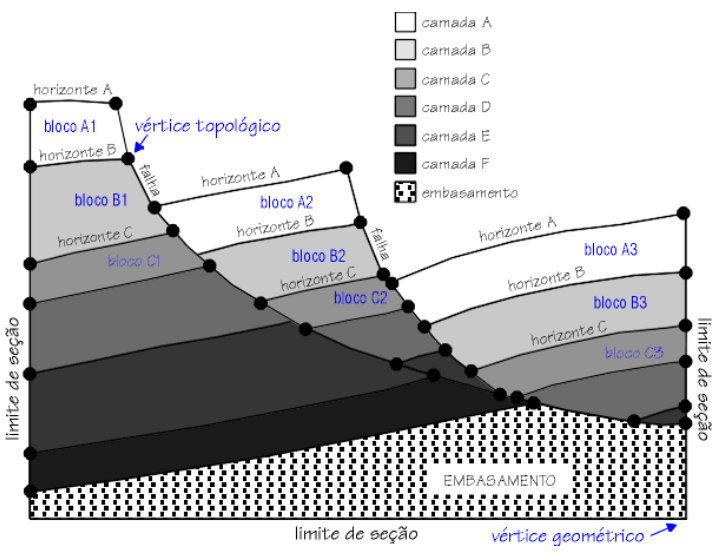
\includegraphics[width=400pt]{images/fig-subdivisao-planar}
    \caption{Seção geológica como uma subdivisão planar.}\label{fig-subdivisao-planar}
  \end{center}
\end{figure}

Uma subdivisão planar pode ser definida como uma subdivisão do plano através do uso de \textit{arestas}, \textit{vértices} e \textit{faces}. Essas são as entidades topológicas presentes em uma subdivisão planar, a face é como a região descrita anteriormente, delimitada por arestas (segmentos de curva); os vértices são os limites das arestas, sendo um para cada extremidade (podendo ser o mesmo vértice no início e no final da aresta).

A subdivisão planar precisa atender a alguns requisitos em relação às entidades topológicas: não deve haver vértices coincidentes; arestas só podem se cruzar em um vértice e faces também só se cruzam ou em um vértice, ou em uma aresta. Em outras palavras, não deve existir sobreposição de elementos topológicos. 

No entanto, há ainda um último componente topológico: o \textit{loop} ou \textit{laço} que é, de forma sucinta, um suconjunto conexo e ordenado de arestas. Com essa definição, a \textit{face} pode ser interpretada como uma união de laços, um deles sendo externo (delimitando a fronteira externa da face) e zero ou mais internos.

Em suma, a subdivisão planar tem os seguintes elementos topológicos:
\renewcommand{\labelitemi}{•}
\begin{itemize}
  \item \textbf{Vértice}: representa um ponto único dentro do plano.
  \item \textbf{Aresta}: segmento de curva com vértices como limites.
  \item \textbf{Laço} (loop): suconjunto conexo e ordenado de arestas.
  \item \textbf{Face}: região delimitada por um ou mais laços.
\end{itemize}

\subsection{Modelagem da Subdivisão Planar}

Para modelar a subdivisão planar dentro do Recon é utilizada a biblioteca computacional \textbf{HED} desenvolvida pelo Instituto Tecgraf/PUC-Rio. O HED é uma estrutura de dados topológicos 

\section{Atributos Geológicos}

\section{Seções Geológicas} % Falar da árvore de cenários

\section{Módulos}

\section{Transformações}

\section{Malhas e Resultados}

This is the first chapter

\section{Linhas de Mapeamento}

Um dos recursos presentes no Sistema Recon é a \textbf{linha de mapeamento}, cujo objetivo é auxiliar na interpretação dos resultados gerados na restauração do modelo. Essa linha armazena referências a pontos topológicos da malha da seção. Com isso, é possível ter uma linha que acompanha a movimentação da malha de um cenário a outro.

As linhas de mapeamento (Figura~\ref{fig-linemap}) permitem realizar um mapeamento geométrico ao longo de uma restauração tomando como base uma linha-guia poligonal definida em um dado cenário. Essa linha pode ser criada em qualquer cenário, mesmo em seções já restauradas.

\begin{figure} [h]
  \begin{center}
    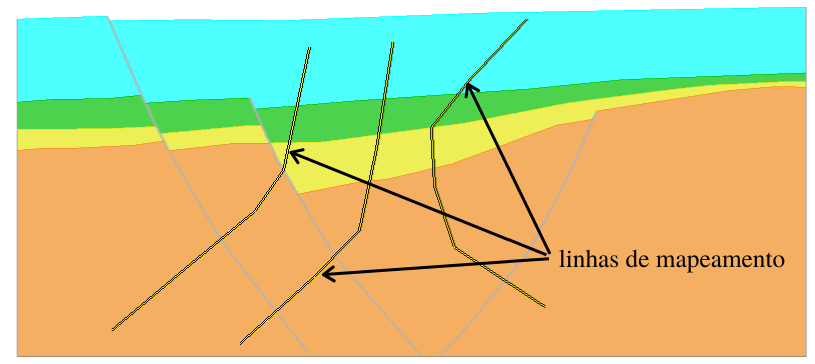
\includegraphics[width=400pt]{images/fig-linhas-de-mapeamento-ed}
    \caption{Linhas de mapeamento em uma seção.}\label{fig-linemap}
  \end{center}
\end{figure}

Cada face de uma seção tem como atributo uma malha triangulada, e as linhas de mapeamento são definidas no sistema de coordenadas local da malha de cada uma das faces. Além disso, é possível que uma linha de mapeamento cruze diversas malhas, por isso, a linha de mapeamento é definida como um conjunto de "partes" de linha de mapeamento, sendo cada parte pertencente a um trecho contínuo em uma mesma face. O processo de criação do mapeamento da linha é feito para cada parte. Na Figura~\ref{fig-linemap-malhas} é possível ver uma linha de mapeamento cortando algumas malhas diferentes.

\begin{figure} [h]
  \begin{center}
    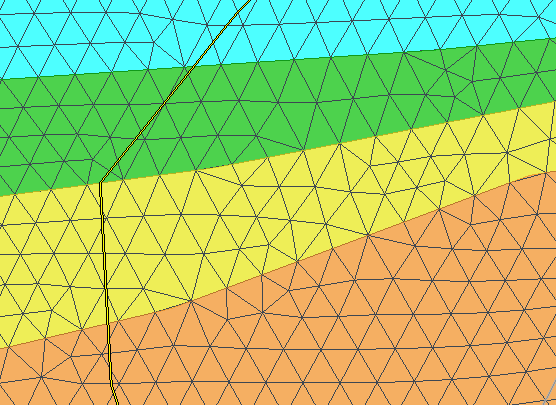
\includegraphics[width=350pt]{images/fig-linhas-de-mapeamento-malhas}
    \caption{Linhas de mapeamento cortando múltiplas faces.}\label{fig-linemap-malhas}
  \end{center}
\end{figure}

A primeira etapa desse mapeamento é a criação da linha-guia, a partir disso é feita a separação nas partes a serem processadas. É realizado um mapeamento com informações topológicas da interseção da parte com a malha. Essa ação consiste em fazer uma relação entre um ponto da parte da linha-guia e um ponto em uma entidade topológica da malha.

Por exemplo, na Figura~\ref{fig-linemap-parts} estão evidenciadas as partes que formam a linha de mapeamento. Cada uma dessas partes é representada pela entidade chamada \textit{LineMapPart}.

\begin{figure} [h]
  \begin{center}
    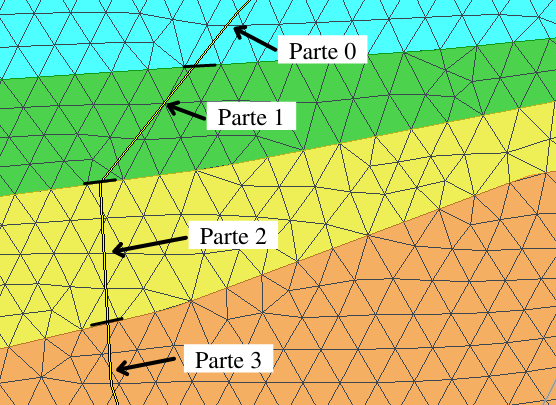
\includegraphics[width=350pt]{images/fig-lm-parts}
    \caption{Partes de uma linha de mapeamento}\label{fig-linemap-parts}
  \end{center}
\end{figure}

Cada parte é processada individualmente e, como já citado, a linha de mapeamento final é um conjunto dessas partes.

Como a malha possui três entidades básicas, o ponto da linha pode ser mapeado para um nó topológico, para um ponto interno de uma aresta (lado de triângulo) de uma malha ou ponto interior a um elemento (triângulo da malha). Em cada um desses casos, a informação topológica relacionada é guardada:

\renewcommand{\labelitemi}{•}
\begin{itemize}
  \item Nó: guarda o indentificador do nó
  \item Aresta: guarda o identificador da aresta e a coordenadas paramétricas do ponto em que cruza a aresta.
  \item Elemento: guarda o identificador do elemento e as coordenadas baricêntricas do ponto no interior do elemento.
\end{itemize}

A Figura~\ref{fig-lm-topo} mostra a idenficação dos pontos da linha de mapeamento e a Tabela~\ref{tab-lm-topo} exibe quais informações topológicas são salvas de cada ponto.

\begin{figure} [hbt!]
  \begin{center}
    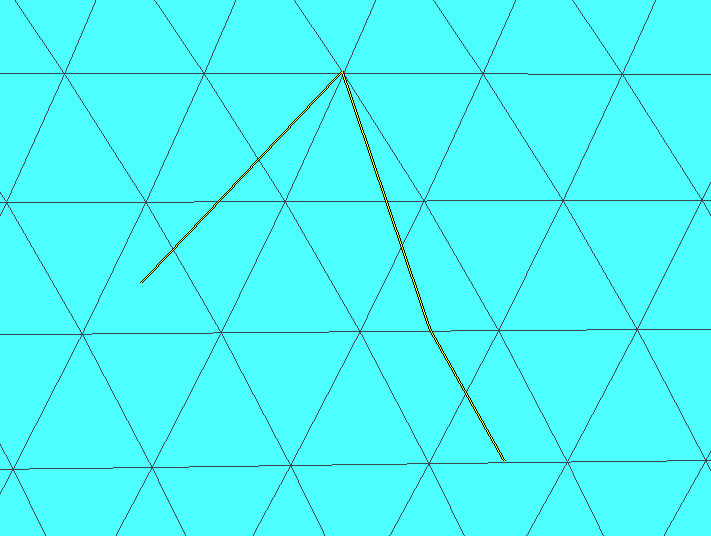
\includegraphics[width=260pt]{images/fig-lm-topo}
    \caption{Informações topológicas da malha mapeadas para a linha de mapeamento.}\label{fig-lm-topo}
  \end{center}
\end{figure}

% -*- coding: utf-8; -*-

\begin{table} [hbt!]
 \begin{center}
	 \caption{Informações topológicas salvas na linha de mapeamento.\label{tab-lm-topo}}
	~\\[-2mm]
	 \begin{tabularx}
		 {\textwidth}
		 {cp{2.0cm} lp{3.0cm} lp{10.0cm}}

		 \textbf{Ponto}
		 & \textbf{Tipo}
		 & \textbf{Informação armazenada} \\ \toprule

		 %~\\[-1mm]
		 A
		 & Elemento
		 & id=30, coordenadas baricêntricas=(0,33; 0,33; 0,33) \\ \midrule

		 %~\\[-1mm]
		 B
		 & Nó   
		 & id=431 \\ \midrule

		 %~\\[-1mm]
		 C
		 & Aresta
		 & id=130, coordenada paramétrica=0,45 \\ \midrule

		 %~\\[-1mm]
		 D
		 & Aresta
		 & id=145, coordenada paramétrica=0,55 \\ \midrule

	 \end{tabularx}
 \end{center}
\end{table}


Após esse processo de mapeamento topológico da linha propriamente dita, é possível calcular a geometria da linha em diferentes cenários que usam a mesma malha (já que a topologia é mantida), bastando apenas verificar se a malha se manteve, isto é, não foi refeita, apagada ou editada.

Em casos de edição, todos os atributos associados à malha são interpolados oara a nova versão da malha, incluem-se nisso as partes de linha de mapeamento que recebem uma nova versão se a malha original teve sua topologia alterada.

A vantagem deste tipo de mapeamento é ser baseado em malha, já que todas as transformações geológicas que ocorrem no processo de restauração, tem como objetivo deformar a malha.

\section{Derivações das Linhas de Mapeamento}

As linhas de mapeamento têm também casos de usos mais especializados, como na criação e representação de poços. Poços são criados semelhantemente às linhas de mapeamento ou por importação de modelos com poços em 3D. Têm característica de serem linhas mais verticalizadas e possuem uma finalidade mais limitada. Nos casos de poços 3D, a linha correspondente ao poço é apenas uma projeção do objeto tridimensional.

Há o uso nas chamadas linhas de interseção (\textit{CrossLine}) que servem para identificar e mapear as linhas de cruzamento entre seções no espaço tridimensional do multi-seções, com isso é possível ter uma noção do que ocorre com seções transversais mesmo estando no domínio bidimensional da restauração.

Por fim, as linhas de mapeamento são a base para a \textit{linhas de mapeamento do modelo} ou \textit{LMModel}, cujo objetivo é servir como um mapeamento das linhas de entidades geológicas (horizonte, falha e topo de sal) ao longo da restauração do modelo. Dessa forma, é possível ter um acompanhamento das entidades geológicas na seção, baseado no contorno da malha das faces que são mais bem discretizadas que as arestas originais da subdivisão planar, além de poder verificar como se deu a movimentação de cada ponto de horizonte ao longo da restauração, por exemplo.

Pelo objetivo proposto, as LMModels são linhas de mapeamento que tomam a geometria das entidades geológicas como entrada, então não há necessidade de criar uma linha-guia como é feita na linha de mapeamento original. Neste caso, há uma parte de LMModel para cada aresta, seja de horizonte, falha ou topo de sal.

Além disso, há o armazenamento de atributos importantes para a manipulação das LMModels, como idade dos horizontes, identificador da falha e até sobre a qual pedaço de superfície aquela parte de linha está associada.

Todas essas informações  geológicas atreladas ao mapeamento topológico das LMModels, quando em conjunto com as diversas seções geológicas de um modelo multi-seções, são o que fazem dela o principal dado para a realização de uma restauração e um mapeamento de informações a nível 3D, já que trazem todo o histórico de movimentação das camadas de um modelo geológico.

A maneira de trabalhar com LMModels é com a organização dela em estruturas de dados que formam subconjuntos divididos por etapa de resturação e idade (caso de linhas de horizonte). Com isso é obtido o conjunto de informações que representam a restauração das seções de uma forma mais simples e fácil de se trabalhar a nível tridimensional.


